\documentclass[a4paper]{article}

% Linguagem
\usepackage[utf8]{inputenc}
\usepackage[portuguese]{babel}
\usepackage[T1]{fontenc}

% Pacotes matemáticos
\usepackage{amsmath}
\usepackage{amsfonts}
\usepackage{amssymb}
\usepackage{graphicx}

% Fontes e identaçãp
\usepackage{setspace}                   % espaçamento flexível
\usepackage{indentfirst}                % indentação do primeiro parágrafo
\usepackage[fixlanguage]{babelbib}
\usepackage[font=small,format=plain,labelfont=bf,up,textfont=it,up]{caption}

% Pacotes para cores e modelos
\usepackage[a4paper,top=3.0cm,bottom=2.0cm,left=3.0cm,right=2.0cm]{geometry} \usepackage[usenames,svgnames,dvipsnames]{xcolor}
\usepackage[pdftex,plainpages=false,pdfpagelabels,pagebackref,
            colorlinks=true,citecolor=DarkGreen,linkcolor=DarkRed,
            urlcolor=DarkRed,filecolor=DarkGreen,
            bookmarksopen=true]{hyperref}

% Pacotes para itens
\usepackage{calc}  
\usepackage{enumitem}  

\title  {Projeto de Laboratório de Programação II - Fase 4}
\author {Karina Suemi, Vinícius Silva, Renato Cordeiro}
\date   {}

%%%%%%%%%%%%%%%%%%%%%%%%%%%%%%%%%%%%%%%%%%%%%%%%%%%%%%%%%%%%%%%%%%%%%%%%

\begin{document}

\maketitle

\bigskip
\bigskip
\bigskip
\bigskip

{\textcolor{NavyBlue}{\Huge{....... MANUAL DO USUÁRIO .......}}


\newpage

     
{\textcolor{NavyBlue}{\LARGE JOGO }

\bigskip

O  jogo consiste  em programar uma  série de 
robôs para batalharem, num estilo de RTS 2x2.
Para  tanto,  os robôs devem  ter suas ações 
programadas. Eles irão executá-las até que o 
jogo acabe ou sejam destruídos.

Nesta fase do desenvolvimento, a programação 
deve ser feita em uma linguagem desenvolvida
especificamente para esse jogo.

Os programas devem  ser criados com extensão 
*.pos*.   Exemplos   estão   disponíveis  no 
diretório `test/` junto ao código-fonte.

\bigskip
\bigskip
\bigskip
\bigskip

{\textcolor{NavyBlue}{\LARGE INSTALAÇÃO }
                
\bigskip
                                            
\textcolor{NavyBlue}{-- 1º PASSO --}

Antes de mais nada, verifique se seu computador possui
o Ant instalado, caso não possua, faça o seguinte:

\begin{enumerate}
    \item Abra o terminal

    \item Digite: \texttt{sudo apt-get install ant}
\end{enumerate}

\bigskip



\textcolor{NavyBlue}{-- 2º PASSO --}

Instalação do ivy:

\begin{enumerate}
    \item Abra o terminal

    \item Entre na pasta (MAC0242-PROJECT)

    \item Digite: \texttt{sudo bash install\_ivy.bash} para uma instalação
          de sistema ou \texttt{bash install\_ivy.bash} para a
          instalação de usuário.
    
\end{enumerate}

\bigskip


\textcolor{NavyBlue}{-- 3º PASSO --}

Para compilar o jogo:

\begin{enumerate}
    \item Ainda com o terminal aberto

    \item Entre na pasta onde está localizado o arquivo do jogo (MAC0242-PROJECT)

    \item Digite \texttt{ant}
\end{enumerate}

\bigskip



\textcolor{NavyBlue}{-- 4º PASSO --}

E para iniciar o jogo: 

\begin{enumerate}                                            
    \item Continuar no terminal
 	\item Digite: \texttt{java -jar dist/MAC0242-Project.jar
          programa1.pos programa2.pos programa3.pos}
\end{enumerate}

Observação: Na pasta "behaviors" você pode encontrar exemplos de 
programas de robô para testar.
Eles são "Carrier.pos" e "Protector.pos".

\bigskip

\newpage %%%%%%%%%%%%%%%%%%%%%%%%%%%%%%%%%%%%%%%%%%%%%%%%%


{\textcolor{NavyBlue}{\LARGE Usando a barra de Menu}

\bigskip
\bigskip
\bigskip

Os botões da lateral direita da tela têm as seguintes
funções:

\bigskip

\begin{itemize}    
                                        
    \item \textcolor{NavyBlue}{MiniMap :}
        Habilita/Desabilita a janela do mini mapa.
    \bigskip
    
 	\item \textcolor{NavyBlue}{Add Robot :}
 	    Ao clicar nesse botão um robô é criado.
 	    
 	    Primeiramente ele pergunta o nome do robô
 	    ser criado.
 	    
 	    Depois, caso o editor de texto esteja vazio
 	    ou desabilitado, ele pede um nome de programa
 	    já criado, para que ele possa comandar o robô.
 	    
 	    Caso o contrário, ele irá carregar o programa
 	    que foi digitado no editor de texto e salvá-lo
 	    na pasta user/ .
    \bigskip
     	    
 	\item \textcolor{NavyBlue}{Editor :}
 	    Habilita/Desabilita a janela do editor de texto.
 	\bigskip
 	
 	\item \textcolor{NavyBlue}{Clear :}
 	    Limpa o editor de texto.
 	\bigskip
 	    
 	\item \textcolor{NavyBlue}{Exit :}
 	    Sair do jogo.
 	\bigskip
 	    
 	\item \textcolor{NavyBlue}{Exit :}
 	    Clicando nos robôs, abre-se a janela do editor
 	    de texto com o programa do respectivo robô 
 	    clicado.

\end{itemize}


\newpage %%%%%%%%%%%%%%%%%%%%%%%%%%%%%%%%%%%%%%%%%%%%%%%%%
        
        
{\textcolor{NavyBlue}{\LARGE Opções}

Você pode escolher várias formas de jogar A Batalha de Robôs,
sendo que cada uma delas envolve um tipo de cenário diferente.
Entre eles temos:

\begin{itemize}
	\item Artical
	\item Tropical
	\item Desertic
	\item Continental
\end{itemize}

Para jogar cada um deles, basta iniciar o programa do seguinte modo:

\begin{itemize}

	\item Artical --> \begin{verbatim}java -jar dist/MAC0242-Project.jar programa1 programa2 programa3 --artical\end{verbatim}

	\item Continental --> \begin{verbatim}java -jar dist/MAC0242-Project.jar programa1 programa2 programa3 --continental\end{verbatim}
	
	\item Desertic --> \begin{verbatim}java -jar dist/MAC0242-Project.jar programa1 programa2 programa3 --desertic\end{verbatim}
	
	\item Tropical --> \begin{verbatim}java -jar dist/MAC0242-Project.jar programa1 programa2 programa3 --tropical\end{verbatim}

\end{itemize}


\newpage %%%%%%%%%%%%%%%%%%%%%%%%%%%%%%%%%%%%%%%%%%%%%%

{\textcolor{NavyBlue}{\LARGE exemplos:}

\bigskip

\begin{figure}[h]
	\centering
    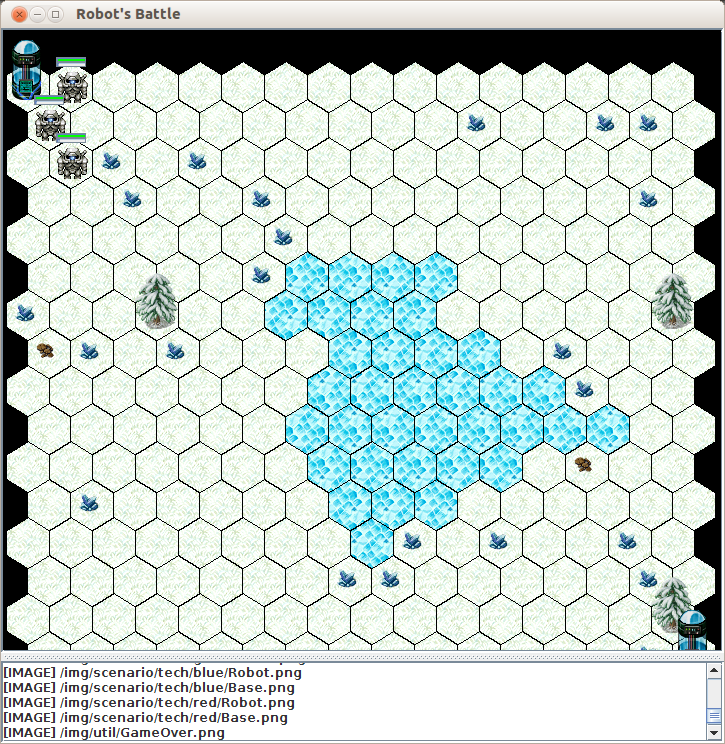
\includegraphics[scale=0.3]{img/artical.png}
    \caption{Artical}
\end{figure}

\bigskip

\begin{figure}[h]
   	\centering
    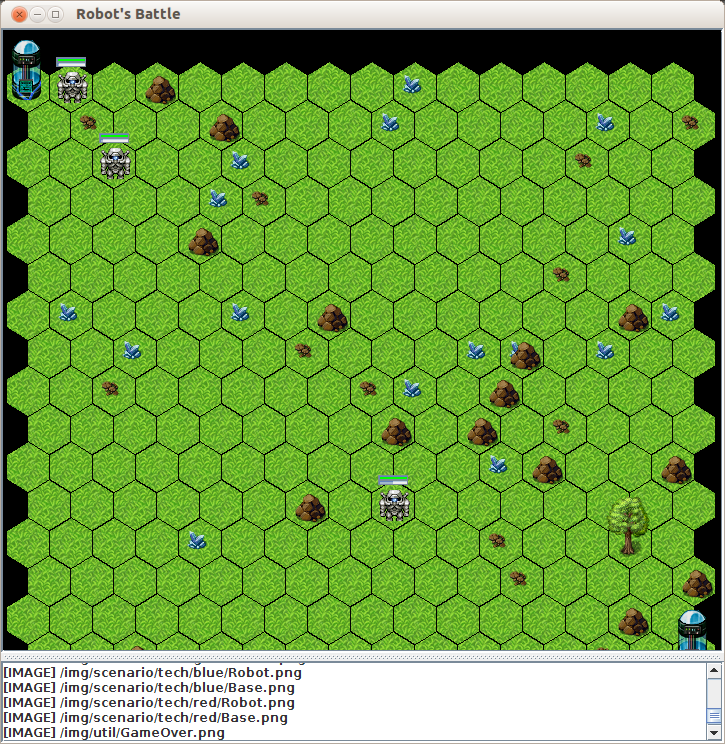
\includegraphics[scale=0.3]{img/continental.png}
    \caption{Continental}
\end{figure}

\newpage %%%%%%%%%%%%%%%%%%%%%%%%%%%%%%%%%%%%%%%%%%%%%%

\begin{figure}[h]
   	\centering
    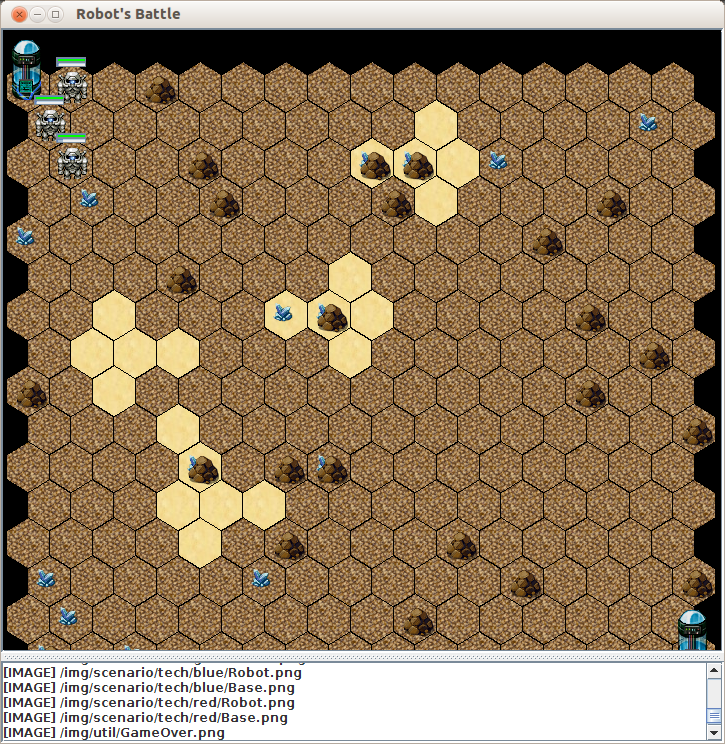
\includegraphics[scale=0.3]{img/desertic.png}
    \caption{Desertic}
\end{figure}

\begin{figure}[h]
   	\centering
    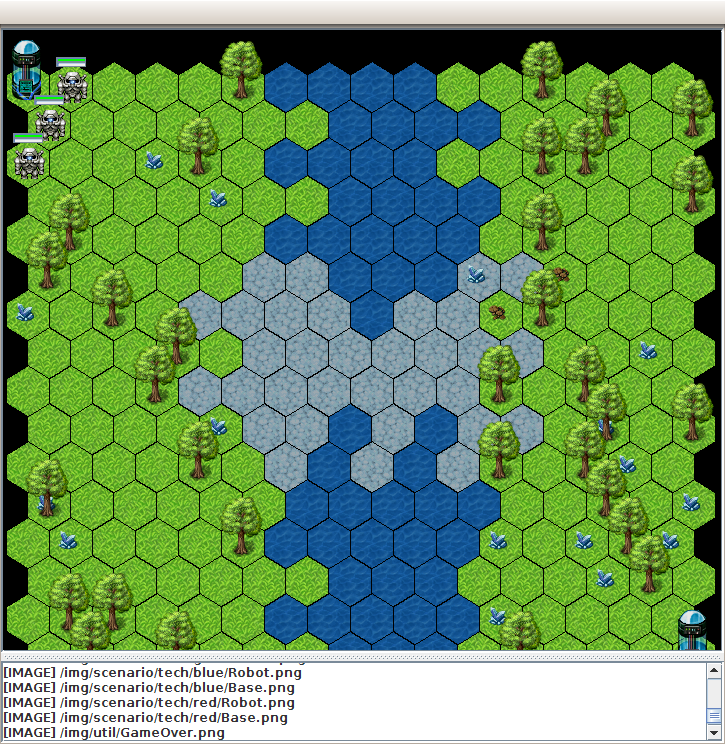
\includegraphics[scale=0.3]{img/tropical.png}
    \caption{Tropical}
\end{figure}

\newpage %%%%%%%%%%%%%%%%%%%%%%%%%%%%%%%%%%%%%%%%%%%%%%

{\textcolor{NavyBlue}{\LARGE Utilitários}
\begin{itemize}

	\bigskip

	\item Se quiser modificar o tamanho da arena,
	coloque "-large" ao final do comando que inicia
	o programa:
	
	\$ \textit {java -jar dist/MAC0242-Project.jar programa1 programa2 programa3 --artical -large}

	\bigskip

	\item E caso queira executar o programa em modo 
	Debugger, digite:

	\$ \textit {java -jar dist/MAC0242-Project.jar }
    	  programa\_jogador\_1 programa\_jogador\_2 -v

	\bigskip
\end{itemize}



\newpage %%%%%%%%%%%%%%%%%%%%%%%%%%%%%%%%%%%%%%%%%%%%%%



{\textcolor{NavyBlue}{\LARGE Guia de Linguagem}

    \bigskip
    \bigskip
    
    Se não quiser utilizar os programas já feitos
    que estão sendo disponibilizados na pasta "test",
    você pode programar seus próprios robôs utilizando
    uma linguagem um tanto quanto simples que é baseada
    no estilo das linguagens de programação mais 
    populares. 
    
    Obs.: No inicio de cada programa, escreva
    {\textcolor{NavyBlue}{updateVars();} 
    para que todas as funções da biblioteca padrão funcionem 
    normalmente.
    
    Para isso, aprenda como essa linguagem funciona:
    
    \begin{itemize}
        
        \item \textbf{Final de um comando :}
        
            No fim de um comando, deve-se colocar 
            \textcolor{NavyBlue}{;}
            .
        
            \textcolor{NavyBlue}{Ex.:} variavel = 2
            \textcolor{NavyBlue}{;}
        
        \bigskip
        
        \item \textbf{Cometários :}
            
            Uma linha de comentário é seguida de 
            \textcolor{NavyBlue}{//}.
            
            \textcolor{NavyBlue}{Ex.:}
            
            // Esse é o comentário!
       
       \bigskip
       
        \item \textbf{Declaração de variáveis :}
        
            Para uma variável ser inicializada, deve-se
            sempre colocar um 
            \textcolor{NavyBlue}{my},
            para variáveis locais ou 
            \textcolor{NavyBlue}{our},
            para variáveis globais,
            antes de seu nome.
            
            \textcolor{NavyBlue}{Ex.:}
            \textcolor{NavyBlue}{my} 
            variavel;
        
            \textcolor{NavyBlue}{Ex.:} 
            \textcolor{NavyBlue}{our} variavel = 2;  
        
        \bigskip
        
        \item \textbf{Atribuição :}
        
            Quando queremos atribuir algum valor a
            determinada variável, basta fazer usar 
            \textcolor{NavyBlue}{=}.
            Também pode-se atribuir um valor a uma
            variável em sua declaração.
            
            \textcolor{NavyBlue}{Ex.:}
            variável 
            \textcolor{NavyBlue}{=}
            42;
            
        \bigskip
        
        \item \textbf{Imprimir - PRINT : }
        
            Para imprimir, é necessário usar o
            comando 
            \textcolor{NavyBlue}{print} e
            colocar o que se deseja imprimir entre
            parênteses.
            Você pode imprimir uma "String" ou o 
            valor de uma variável.
            
            \textcolor{NavyBlue}{Ex.:}
            \textcolor{NavyBlue}{print(variavel)}
            ;
            
            \textcolor{NavyBlue}{Ex.:}
            \textcolor{NavyBlue}{print("Hello World!")}
            ;
       
       \bigskip
            
       \item \textbf{Imprimir - SAY : }
        
            Para imprimir, é necessário usar o
            comando 
            \textcolor{NavyBlue}{say} e
            colocar o que se deseja imprimir entre
            parênteses.
            Você pode imprimir uma "String" ou o 
            valor de uma variável.
            A diferença entre SAY e PRINT é que
            SAY pula uma linha no fim e PRINT não.
            
            \textcolor{NavyBlue}{Ex.:}
            \textcolor{NavyBlue}{say(variavel)}
            ;
            
            \textcolor{NavyBlue}{Ex.:}
            \textcolor{NavyBlue}{say("Hello World!")}
            ;
        
            
\newpage %%%%%%%%%%%%%%%%%%%%%%%%%%%%%%%%%%%%%%%%%%%%%%%%%%%%%%%%%%%
            
            
        \item \textbf{IF | ELSE | ELSIF : }
            
            Para uma condição inicial, usamos
            \textcolor{NavyBlue}{if},
            para uma segunda condição, caso a 
            primeira não ocorra, usamos
            \textcolor{NavyBlue}{elsif}
            e quando nenhuma das ações ocorra
            usamos 
            \textcolor{NavyBlue}{else}.
            
            \textcolor{NavyBlue}{Ex.:}
            
            \textcolor{NavyBlue}{if(a>b)}
            
            \{
            
            \ \ \ \  say("a é maior");
            
            \}
            
            \textcolor{NavyBlue}{elsif(a == b)}
            
            \{
            
            \ \ \ \ say("a é igual a b");
            
            \}
            
            \textcolor{NavyBlue}{else}
            
            \{
            
            \ \ \ \  say("a é menor a b");
            
            \}
    
        \bigskip    
            
        \item \textbf{WHILE :}
            
            O while é utilzado normalmente, quando se
            deseja ter um laço, o usamos com a condição
            entre parêntesis.
        
            \textcolor{NavyBlue}{Ex.:}
            
            \textcolor{NavyBlue}{while(a<5)}
            
            \{
            
            \ \ \ \  say("Hello!!");
            \ \ \ \  a = a+1;
            
            \}
        
        \bigskip
            
        \item \textbf{BREAK :}
            
            Break é um auxiliar do While usado quando se 
            deseja parar o loop.
            
            \textcolor{NavyBlue}{Ex.:}
            
            while(k<5)
            
            \{
            
            \ \ \ \ if(k == 1)
              
            \ \ \ \ \{
              
            \ \ \ \ \ \ \ \ \textcolor{NavyBlue}{break}
                    ;
              
            \ \ \ \ \}
           
            \}
        
\newpage %%%%%%%%%%%%%%%%%%%%%%%%%%%%%%%%%%%%%%%%%%%%%%%%%%%%%%%%%%%%%
            
        \item \textbf{CONTINUE :}
            
            Continue também é um auxiliar do while que é
            usado quando se deseja pular tudo o que vem
            depois do continue e continuar com o laço.
            
            \textcolor{NavyBlue}{Ex.:}
            
            while(k<5)
            
            \{
            
            \ \ \ \ if(k == 1)
              
            \ \ \ \ \{
              
            \ \ \ \ \ \ \ \ \textcolor{NavyBlue}{break}
                    ;
              
            \ \ \ \ \}
           
            \}
        
        \bigskip   
                           
        \item \textbf{FUNÇÕES :}
            
            Nas linguagens de programação usuais, vemos a
            presença de funções.
            Não sendo diferente delas, essa linguagem também
            utiliza funções para facilitar o modo de programação.
            Poré possui as seguintes restrições:
                       
            \begin{enumerate}
                
                \item Para declarar a função, usamos 
           	        \textcolor{NavyBlue}{def}, tipo de retorno, nome
            	    da função e (tipo de parâmetros)
            	
                	\textcolor{NavyBlue}{Ex.:}
                	
                	\textcolor{NavyBlue}{def}
                	number square(number);
                	
            	\bigskip

                \item Para chamá-la usamos
                    o nome da função e seus parâmetros entre 
                    parênteses, em ordem.
                    
                    \textcolor{NavyBlue}{Ex.:}
                    
                    hSquared = square(catA);
                
                \bigskip
                
                \item Para contruí-las basta usar  o tipo
                    de retorno + o nome da função e entre
                    parênteses os nomes dos parâmetros acompanhados de 
                    seus respectivos tipos. Tudo isso seguido da ação que
                    ela irá realizar entre chaves {}.
                    
                    Não esquecendo de dar
                    \textcolor{NavyBlue}{return}
                    nas funções que retornam algum tipo de dado.
                    
                    \textcolor{NavyBlue}{Ex.:}
                    
                        number square(number x)
                        
                        \{
                        
                        \ \ \ \ my j = x;
                        
                        \ \ \ \ return x*j;
                        
                        \}
                
            \end{enumerate}
            
        \bigskip      
       
        \item \textbf{toCOORD :}
            
            Transforma dois números I e J em coordenadas
        
        \bigskip      
        
        \item \textbf{toNumberI :}
            
            Pega uma coordenada e devolve o número relacionado
            a posição I
            
            \textcolor{NavyBlue}{Ex.:}
            
            toNumberI(c);
            
            sendo c uma coordenada.
            
        \bigskip
        
        \item \textbf{toNumberJ :}
            
            Pega uma coordenada e devolve o número relacionado
            a posição J
            
            \textcolor{NavyBlue}{Ex.:}
            
            toNumberJ(c);
            
            sendo c uma coordenada.
            
       
       
\newpage %%%%%%%%%%%%%%%%%%%%%%%%%%%%%%%%%%%%%%%%%%%%%%
        
         
        \item \textbf{ASK}
        
            Para saber onde determinado robô se localiza
            ele deve usar a função 
            \textcolor{NavyBlue}{ask} 
            que retornará a sua posição na forma
            Coordenate.
        
            \textcolor{NavyBlue}{Ex.:}
        
            my c = toCoord(ask("position"));
        
        \bigskip
        
        \item \textbf{HIT}
            
            Para atacar um outro robô é necessário 
            usar o comando
            \textcolor{NavyBlue}{hit},
            ele recebe como parâmetro a direção em
            que se deseja atacar. 
            Essa direção deve ser da forma Direction.
            Devolvendo 1 quando conseguiu atacar o
            alvo naquela direção e 0 caso o ataque
            não tenha sido bem sucedido.
            
            \textcolor{NavyBlue}{Ex.:}
            
            hit(->NW)

        \bigskip
        
        \item \textbf{MOVE}
            
            Para mover um robô de lugar, usa-se o comando
            \textcolor{NavyBlue}{move},
            sendo que este recebe como parâmetro a direção
            em forma de Direction e retorna 1 caso
            tenha andado e 0 caso contrário.
                
            \textcolor{NavyBlue}{Ex.:}

            move(->E)
            
        \bigskip

        \item \textbf{FIRE}
            
            A função 
            \textcolor{NavyBlue}{fire}
            funciona no mesmo estilo de HIT,
            porém essa é para os robôs que tem mais alcance.
            Ao executar essa função, você estará atacando um
            alvo em determinada coordenada, caso o seu alcance
            permita.
            Ele funciona como um tiro normal, caso haja algum
            obstaculo no meio, este será atingido.
            
            Essa função recebe como parâmetro a coordenada em
            que se deseja atacar e devolve 1 caso o ataque tenha
            sido realizado com sucesso e 0 caso contrário,
            lembrando que se o alcance do robô não permitir tal 
            ataque, a função retornará 0 e o ataque não será
            executado.
            
            \textcolor{NavyBlue}{Ex.:}
            
            fire([12,15]);

        \bigskip
        
        \item \textbf{LOOK}
        
            Essa função procura por algum item (como por exemplo
            o cristal).
            Quando usamos 
            \textcolor{NavyBlue}{look},
            precisamos de um parâmetro do tipo Item que se refere
            ao tipo de objeto que estejamos procurando.
            Em seu retorno, obtemos a coordenada do objeto encontrado.

            \textcolor{NavyBlue}{Ex.:}
            
            x = look( %stone );
        
        \bigskip
        
        \item \textbf{DRAG}
        
            Para coletar algo do mapa, deve-se utilizar
            \textcolor{NavyBlue}{drag},
            essa função irá retornar 1 se o objeto foi
            coletado e 0 caso contrário.
            E como parâmetro é passada a direção em forma
            de Direction;

            \textcolor{NavyBlue}{Ex.:}
            
            drag(->NW);

        \bigskip
                
        \item \textbf{DROP}
        
            Para soltar algo no mapa, deve-se utilizar 
            a função
            \textcolor{NavyBlue}{drop},
            ela irá retornar 1 se o objeto for solto com
            e 0 caso isso não tenha dado certo.
            E deve receber como parâmetro uma direção
            em forma de Direction.

            \textcolor{NavyBlue}{Ex.:}
            
            drop(->E);
            
        \end{itemize}

\newpage %%%%%%%%%%%%%%%%%%%%%%%%%%%%%%%%%%%%%%%%%%%%%%%%%%%%%%%%%%%%


{\textcolor{NavyBlue}{\LARGE Tipos de Variáveis}

    \bigskip
    \bigskip
    
    Temos os tipos:
        
    \begin{itemize}
        
        \item \textcolor{NavyBlue}{Item:} Itens como rocha e cristal
            
            \%item
            
            \textcolor{NavyBlue}{Ex.:} \%stone
                
        \bigskip
        
        \item \textcolor{NavyBlue}{Number:} Números
            
            -- número normal --
            
            \textcolor{NavyBlue}{Ex.:} 4242
            
        \bigskip            
            
        \item \textcolor{NavyBlue}{String:} Variáveis texto
            
            "mensagem"
            
            \textcolor{NavyBlue}{Ex.:} "Hello"         
        
        \bigskip
                         
        \item \textcolor{NavyBlue}{Direction:} Direções como leste, 
        oeste, nordeste, entre outros.
            
            ->direção
            
            \textcolor{NavyBlue}{Ex.:} ->NE
        
        \bigskip
        
        \item \textcolor{NavyBlue}{Coordinate:} Coordenas da representação
        quadrada da matriz diagonal.
            
            [I,J]
            
            \textcolor{NavyBlue}{Ex.:} [4,2]
            
    \end{itemize}
    
\newpage %%%%%%%%%%%%%%%%%%%%%%%%%%%%%%%%%%%%%%%%%%%%%%

\bigskip
\bigskip
\bigskip
\bigskip

{\textcolor{NavyBlue}{\LARGE DOCUMENTAÇÃO }

A   documentação    do   código-fonte   está 
disponível no formato Javadoc e no formato 
de relatório Latex para compreendimento do 
código.

\end{document}
